\subsubsection{Multi-session models: transferring interpretations across sessions}
\label{subsubsection:rebuttal_multisession}

\paragraph{Multi-session SED.}
Units recorded in different sessions do not correspond: each Aeon recording block is spike-sorted separately, and other animals have different units altogether. A multi-session TW-SED therefore gives every session $s$ its own linear input mapping $E_s$ from that session's $N_s$ units to the Transformer's token space, and its own decoder $W_s$ from the latents back to the same units (\autoref{fig:rebuttal_multisession_schematic}). The temporal core (the self-attention layers and the projection to the latents) and the $D$ latents are shared by all sessions. A session may also own $P$ session-specific latents, read out from the same core and appended after the shared latents as an outermost Matryoshka level $(D+P,\,k+k_P)$. The shared levels must still reconstruct the session on their own, so session-specific latents take up only what the shared latents leave unexplained.

Data handling follows the single-session pipeline. Counts are standardized within each session, windows are built within a session and never cross a session boundary, every batch comes from one session, and training and evaluation splits can be made by whole session. Sessions can be trained jointly from scratch. Alternatively, a trained model can be extended to a new session by freezing all existing parameters and training only the new session's input mapping, decoder, and session-specific latents on that session's neural activity. We use this second mode here, because it leaves the session A model of \autoref{subsection:aeon_results}, and therefore every interpretation already made with it, unchanged.

\begin{figure}[!htbp]
    \centering
    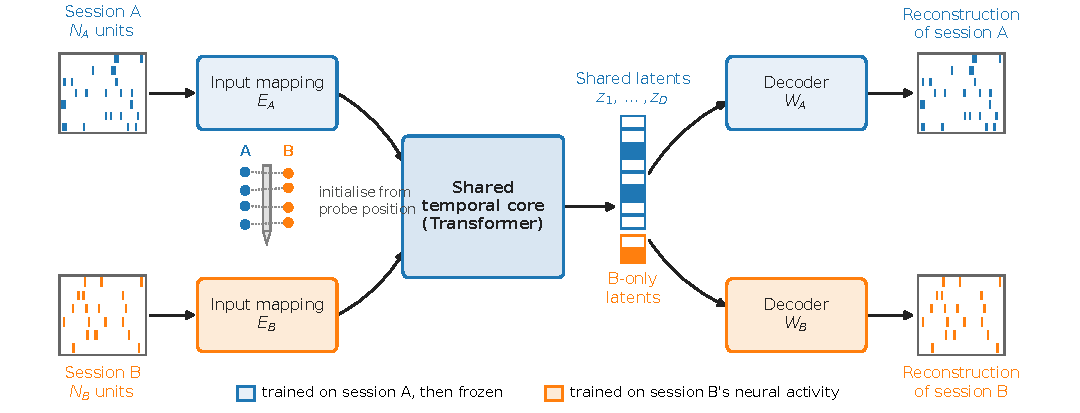
\includegraphics[width=\linewidth]{figures/rebuttal/change02_multisession/multisession_schematic.pdf}
    \caption{\textbf{Multi-session SED.} Each session has its own input mapping and decoder around a shared temporal core and shared latents; a session can add a few session-specific latents. To transfer a trained model, the session A components (blue) are frozen and the session B components (orange) are trained to reconstruct session B's neural activity. When both sessions come from the same probe insertion, the session B mappings are initialised from the session A mappings of the units at the nearest probe positions.}
    \label{fig:rebuttal_multisession_schematic}
\end{figure}

\paragraph{Session B.}
Session A is the recording analyzed in \autoref{subsection:aeon_results}. Session B comes from the same mouse and probe insertion, from June 5, 2024, 23:00 to June 6, 17:00, the same 18 clock hours one day earlier, ending six hours before session A begins. Among the other recording blocks of the experiment it matches session A most closely in foraging: 176 food deliveries (181 in session A) and wheel activity in 2.4\% of bins (2.9\%). It is prepared exactly as session A and contains 54,128,107 spikes from 87 Kilosort~4 clusters and 3,238,618 valid windows. The block was sorted separately, so its 87 clusters carry no identities in common with the 90 clusters of session A.

\paragraph{Replication on session B alone.}
We first train new models on session B alone with the settings of \autoref{subsection:aeon_results}. The $D=192$, $k=12$ model again contains a \textit{wheel activity} latent (latent 63, \metric{AUROC} $0.901$), and the $D=256$, $k=12$ model again contains latents for the three supplementary features (\metric{AUROC} $0.839$, $0.829$, and $0.903$). The best-matching latent of these models serves as the reference for what a model fitted directly to session B achieves (\autoref{table:rebuttal_multisession_transfer}).

\paragraph{Transfer protocol.}
We freeze the session A models and add session B with $P=16$ session-specific latents and $k_P=2$, giving levels $(96,6)$, $(192,12)$, and $(208,14)$ for the $D=192$ model and the corresponding levels for $D=256$. Because both sessions use the same probe insertion, the position of a cluster on the probe gives a correspondence between sessions that uses neither neural activity nor behavior. We take each cluster's mean Kilosort spike position and match every cluster to the nearest cluster of the other session (median distance 1.1~$\mu$m; 90th percentile 6.1~$\mu$m). The session B input mapping is initialised so that each session A unit's input weights are driven by its nearest session B unit, and each session B unit inherits the decoder weights of its nearest session A unit. The session B components are then trained for 5,000 Adam updates with the optimization settings of \autoref{subsection:aeon_results}, using session B's neural activity only, after which activation thresholds are calibrated on session B as for any model.

Behavior from session B enters only at scoring. Feature definitions, latent indices, and activation rules are those of session A: latent 52 with $z\geq3.31$ for \textit{wheel activity}, and latents 107, 109, and 10 with $z>0$ for the supplementary features. Quintile boundaries are recomputed on session B, as the definitions specify. Three comparisons calibrate the result: position matching with no training; the same training from a random initialisation of the session B input mapping and decoder; and the same position-based initialisation after randomly permuting which session B unit sits at which probe position. All other shared latents, scored on the same feature, give the chance level.

\paragraph{Transfer results.}
After transfer, latent 52 of the frozen session A model tracks \textit{wheel activity} in session B: \metric{Cov} $0.847$, \metric{Spec} $0.819$, \metric{Sel} $0.824$, \metric{AUROC} $0.893$, against $0.938$, $0.820$, $0.839$, and $0.924$ in session A (\autoref{table:rebuttal_multisession_transfer}). Its activation probability as a function of wheel speed is nearly identical in the two sessions, with the same step at the $0.75$ cm/s boundary (\autoref{fig:rebuttal_multisession_wheel}a,b). It is the highest-scoring of all 192 shared latents, whose \metric{AUROC}s otherwise have median $0.501$ and 95th percentile $0.519$ (\autoref{fig:rebuttal_multisession_wheel}c), and it matches the best latent of the model trained on session B alone ($0.901$). The three supplementary features transfer in the same way: latents 107, 109, and 10 are each the highest-scoring of the 256 shared latents for their feature, with scores and tuning close to session A (\autoref{fig:rebuttal_multisession_latents}). The transferred models reconstruct session B as well as the models trained on it alone (mean squared error on standardized counts $0.770$ versus $0.780$ at $D=192$).

\begin{table}[!htbp]
    \centering
    {\small\setlength{\tabcolsep}{3pt}\renewcommand{\arraystretch}{1.1}
    \begin{tabular*}{\linewidth}{@{\extracolsep{\fill}}lrrrrr@{}}
\toprule
Model and session & Latent & \metric{Cov} & \metric{Spec} & \metric{Sel} & \metric{AUROC} \\
\midrule
\multicolumn{6}{l}{\textit{Wheel activity} ($D=192$, $k=12$)} \\
Session A, paper model & 52 & 0.938 & 0.820 & 0.839 & 0.924 \\
Session B, transferred & 52 & 0.847 & 0.819 & 0.824 & 0.893 \\
Session B, position matching only & 52 & 0.857 & 0.818 & 0.825 & 0.892 \\
Session B, other 191 shared latents & -- & -- & -- & -- & 0.501 (0.519, 0.823) \\
Session B only, best-matching latent & 63 & 0.854 & 0.820 & 0.826 & 0.901 \\
\midrule
\multicolumn{6}{l}{\textit{Smaller area near the patch} ($D=256$, $k=12$)} \\
Session A, paper model & 107 & 0.837 & 0.761 & 0.778 & 0.849 \\
Session B, transferred & 107 & 0.895 & 0.750 & 0.782 & 0.876 \\
Session B, position matching only & 107 & 0.902 & 0.736 & 0.774 & 0.875 \\
Session B, other 255 shared latents & -- & -- & -- & -- & 0.499 (0.547, 0.705) \\
Session B only, best-matching latent & 73 & 0.831 & 0.785 & 0.795 & 0.839 \\
\midrule
\multicolumn{6}{l}{\textit{Highest centroid-speed quintile} ($D=256$, $k=12$)} \\
Session A, paper model & 109 & 0.718 & 0.781 & 0.767 & 0.778 \\
Session B, transferred & 109 & 0.739 & 0.789 & 0.778 & 0.793 \\
Session B, position matching only & 109 & 0.730 & 0.791 & 0.778 & 0.790 \\
Session B, other 255 shared latents & -- & -- & -- & -- & 0.500 (0.566, 0.760) \\
Session B only, best-matching latent & 15 & 0.826 & 0.752 & 0.769 & 0.829 \\
\midrule
\multicolumn{6}{l}{\textit{Radially outward movement} ($D=256$, $k=12$)} \\
Session A, paper model & 10 & 0.840 & 0.805 & 0.812 & 0.872 \\
Session B, transferred & 10 & 0.828 & 0.784 & 0.793 & 0.858 \\
Session B, position matching only & 10 & 0.844 & 0.766 & 0.783 & 0.865 \\
Session B, other 255 shared latents & -- & -- & -- & -- & 0.500 (0.543, 0.660) \\
Session B only, best-matching latent & 48 & 0.984 & 0.345 & 0.600 & 0.903 \\
\bottomrule
\end{tabular*}
}
    \caption{\textbf{Transfer of the paper's four Aeon features to session B.} Rows compare the session A scores of \autoref{table:aeon_feature_metrics} with the same latent of the same frozen model on session B, after training the session B input mapping and decoder (\emph{transferred}) and with position matching alone. \metric{Cov}, \metric{Spec}, and \metric{Sel} use the session A activation rules ($z\geq3.31$ for latent 52, $z>0$ otherwise). ``Other shared latents'' gives the median \metric{AUROC} of the remaining shared latents on the same feature, with the 95th percentile and maximum in parentheses. ``Session B only'' is the best-matching latent (highest \metric{AUROC}) of a model trained on session B alone; its \textit{wheel activity} scores use the activation threshold with the session A false-positive rate.}
    \label{table:rebuttal_multisession_transfer}
\end{table}

\begin{figure}[!htbp]
    \centering
    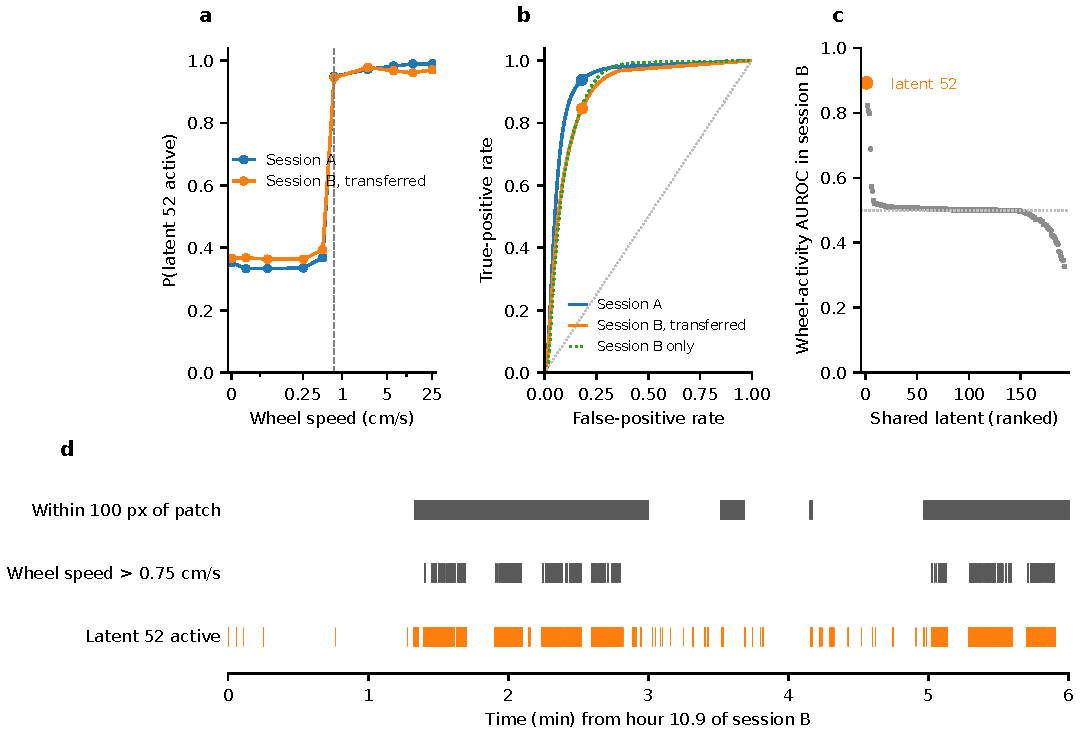
\includegraphics[width=\linewidth]{figures/rebuttal/change02_multisession/multisession_wheel_transfer.pdf}
    \caption{\textbf{The \textit{wheel activity} latent keeps its interpretation in session B.} (\textbf{a}) Activation probability of latent 52 ($D=192$, $k=12$) by wheel speed, in session A and, for the same latent after transfer, in session B; vertical dashed line at $0.75$ cm/s. (\textbf{b}) ROC curves based on latent activations; dots mark the $z\geq3.31$ operating point in both sessions. The dotted curve is the best-matching latent of a model trained on session B alone. (\textbf{c}) \metric{AUROC} for \textit{wheel activity} in session B of each of the 192 shared latents, ranked. (\textbf{d}) A six-minute excerpt of session B: 20-ms bins with centroid position within 100 px of the patch, wheel-rim speed above $0.75$ cm/s, and activation of the transferred latent 52.}
    \label{fig:rebuttal_multisession_wheel}
\end{figure}

\begin{figure}[!htbp]
    \centering
    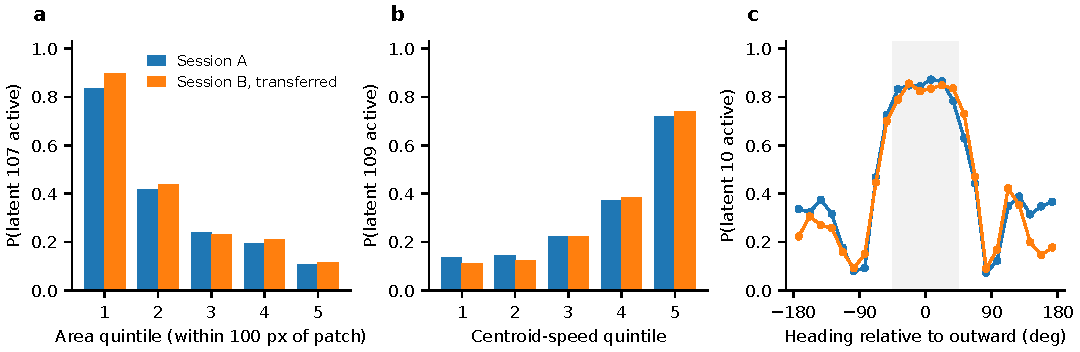
\includegraphics[width=\linewidth]{figures/rebuttal/change02_multisession/multisession_appendix_latents.pdf}
    \caption{\textbf{Tuning of the supplementary latents in sessions A and B.} Activation probability of latents 107 (\textbf{a}), 109 (\textbf{b}), and 10 (\textbf{c}) of the $D=256$, $k=12$ model in session A and, for the same latents after transfer, in session B. Axes and eligible windows follow \autoref{fig:aeon_additional_features} and \autoref{fig:aeon_direction}; shading in (\textbf{c}) marks the scored $\pm45^\circ$ sector.}
    \label{fig:rebuttal_multisession_latents}
\end{figure}

\paragraph{Initialisation and further sessions.}
\autoref{table:rebuttal_multisession_controls} separates the contributions of the frozen core, the probe-position initialisation, and training. Beyond the four selected latents, we score every shared latent against a fixed panel of behavior conditions (quintiles of position, speed, acceleration, area, patch distance, and wheel speed; heading sectors; arena locations; wheel-bout onsets and offsets; and food delivery), and ask, for each condition that some session A latent separates clearly (activation-rate difference of at least $0.3$ inside versus outside the condition), whether that latent is still the best-separating shared latent in the new session.

With probe-position initialisation the result is the same for every training seed, and the best session A latent remains the best latent in session B for 78\% of 60 conditions (top three for 93\%) at $D=192$. Position matching alone, with no training, already places each of the four paper latents first for its feature; training improves reconstruction and the share of conditions that keep their latent. From a random initialisation, the frozen core still assigns some features to their session A latents (the speed latent in every seed, the \textit{wheel activity} latent in one seed of three), but the outcome varies between seeds and the \textit{radially outward} latent is never recovered. Permuting the unit positions before initialisation removes the transfer of the \textit{wheel activity}, area, and direction latents. The interpretation therefore travels with the frozen core and latents, and a correct unit correspondence makes the transfer reliable.

The same procedure applied to a third recording, session E, two days after session A (June 8, 23:00 to June 9, 17:00; 86 clusters, 162 food deliveries), gives the same result: latent 52 is again the highest-scoring shared latent for \textit{wheel activity} (\metric{Cov} $0.907$, \metric{Spec} $0.814$, \metric{Sel} $0.830$, \metric{AUROC} $0.913$).

\begin{table}[!htbp]
    \centering
    {\small\setlength{\tabcolsep}{2.5pt}\renewcommand{\arraystretch}{1.1}
    \begin{tabular*}{\linewidth}{@{\extracolsep{\fill}}llrrrrrrr@{}}
\toprule
 & & & \multicolumn{2}{c}{$D=192$} & \multicolumn{4}{c}{$D=256$} \\
\cmidrule(lr){4-5}\cmidrule(lr){6-9}
Session & Initialisation & Seed & \shortstack{Wheel\\latent 52} & \shortstack{Top-1 / top-3\\(\%)} & \shortstack{Area\\latent 107} & \shortstack{Speed\\latent 109} & \shortstack{Direction\\latent 10} & \shortstack{Top-1 / top-3\\(\%)} \\
\midrule
B & Position & 0 & 0.893 (1) & 80 / 95 & 0.876 (1) & 0.793 (1) & 0.858 (1) & 57 / 85 \\
 &  & 1 & 0.891 (1) & 81 / 93 & 0.877 (1) & 0.793 (1) & 0.858 (1) & 57 / 85 \\
 &  & 2 & 0.893 (1) & 81 / 93 & 0.876 (1) & 0.792 (1) & 0.864 (1) & 57 / 85 \\
 & Position only & -- & 0.892 (1) & 68 / 93 & 0.875 (1) & 0.790 (1) & 0.865 (1) & 57 / 85 \\
 & Random & 0 & 0.899 (1) & 51 / 59 & 0.865 (1) & 0.859 (1) & 0.435 (250) & 41 / 65 \\
 &  & 1 & 0.390 (184) & 36 / 37 & 0.686 (4) & 0.878 (1) & 0.449 (248) & 28 / 39 \\
 &  & 2 & 0.765 (3) & 37 / 58 & 0.371 (251) & 0.834 (1) & 0.658 (2) & 31 / 31 \\
 & Scrambled & 0 & 0.413 (183) & 36 / 42 & 0.428 (249) & 0.807 (1) & 0.270 (256) & 30 / 37 \\
 &  & 1 & 0.530 (14) & 51 / 76 & 0.863 (1) & 0.807 (1) & 0.344 (255) & 52 / 74 \\
 &  & 2 & 0.485 (160) & 47 / 80 & 0.744 (2) & 0.800 (2) & 0.841 (1) & 33 / 56 \\
\midrule
C & Position & 0 & 0.924 (1) & 68 / 93 & 0.847 (1) & 0.756 (1) & 0.837 (1) & 61 / 80 \\
 & Position only & -- & 0.910 (1) & 66 / 89 & 0.852 (1) & 0.751 (1) & 0.845 (1) & 55 / 84 \\
 & Random & 0 & 0.499 (146) & 38 / 39 & 0.506 (28) & 0.804 (1) & 0.490 (234) & 24 / 33 \\
\midrule
D & Position & 0 & 0.913 (1) & 53 / 73 & 0.830 (1) & 0.795 (1) & 0.834 (1) & 56 / 76 \\
 & Position only & -- & 0.895 (1) & 49 / 75 & 0.847 (1) & 0.777 (1) & 0.847 (1) & 52 / 72 \\
 & Random & 0 & 0.482 (171) & 31 / 47 & 0.488 (241) & 0.787 (1) & 0.667 (2) & 26 / 26 \\
\bottomrule
\end{tabular*}
}
    \caption{\textbf{Initialisation controls and a further session.} Feature columns give the \metric{AUROC} in the new session of the session A latent for that feature, with its rank among all shared latents in parentheses. ``Top-1 / top-3'' is the percentage of behavior conditions whose best-separating session A latent is the best, or among the three best, shared latents for the same condition in the new session. All rows except ``no training'' train the new session's input mapping, decoder, and session-specific latents for 5,000 updates on neural activity alone.}
    \label{table:rebuttal_multisession_controls}
\end{table}

\paragraph{A food-delivery feature in session B.}
Inspecting the model trained on session B alone ($D=192$, $k=12$) against behavior and task events reveals a feature that is not among those described for session A: latent 77 is active from about $0.3$ to $1.0$ s after a food-delivery trigger (\autoref{fig:rebuttal_multisession_food}). It responds after all 176 deliveries in the session, and 6,097 of its 6,235 active windows fall within 2 s after a delivery. Scored against the description \textit{food delivery}, defined as $0.3$ to $1.0$ s after a delivery trigger and compared with all other neural-valid windows, it reaches \metric{Cov} $0.952$, \metric{Spec} $0.9999$, \metric{Sel} $0.9999$, and \metric{AUROC} $0.976$. A second latent of the same model (latent 53) covers the first $0.3$ s after the trigger. As with the other Aeon features, this is a descriptive association: the latent may reflect the sound of the dispenser, the arrival of the pellet, or the animal's response to either.

\begin{figure}[!htbp]
    \centering
    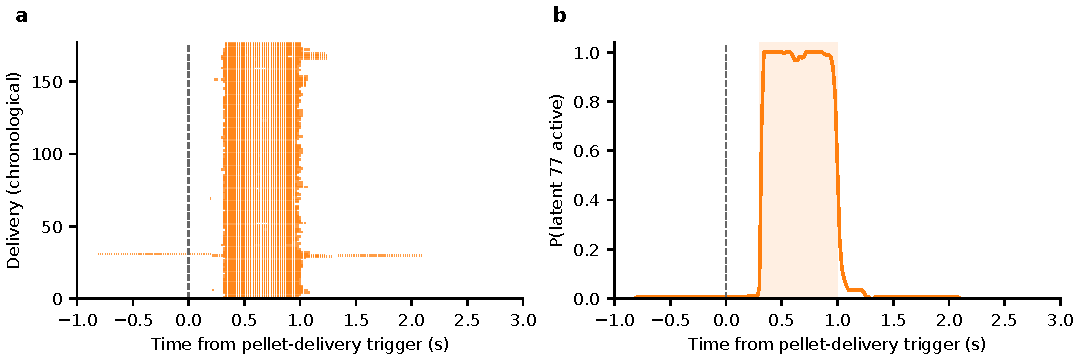
\includegraphics[width=\linewidth]{figures/rebuttal/change02_multisession/multisession_food_delivery.pdf}
    \caption{\textbf{A \textit{food delivery} latent in session B.} Latent 77 of the $D=192$, $k=12$ model trained on session B alone. (\textbf{a}) Windows with positive activation around each of the 176 food-delivery triggers. (\textbf{b}) Activation probability relative to the trigger; shading marks the scored interval, $0.3$ to $1.0$ s.}
    \label{fig:rebuttal_multisession_food}
\end{figure}
